\chapter{The Runtime Library} \label{sec:runtime}
In this chapter, the work performed towards implementing the runtime library is presented. This library handles several core functions critical to the infrastructure of the application:

\begin{itemize}
	\item Functions for collecting trace analyses
	\item Implementations of trace storage backends
	\item Algorithms for offline and online dependency analysis
\end{itemize}

Additionally, tools for generating sample dependency patterns are also included.

The programs described within this chapter are open-source, released under The University of Edinburgh GPL license. They are available at \url{https://github.com/chrisatkin/locomotion}.

The fully-qualified package identifier for the runtime library is\\\texttt{uk.ac.ed.inf.icsa.locomotion.instrumentation}.

\section{Trace Collection} \label{sec:runtime/trace-collection}
One of the main functionalities of the runtime library is to enable the collection of traces. This entails logging all appropriate memory operations (i.e., the ones matching conditions presented in \ref{items:reqs}), with some additional semantic information which is also required.

The user-facing functions for trace collection have the following signatures:

\begin{verbatim}
public static <T> void
arrayLookup(T[] array, int index, int iterator, int id);

public static <T> void
arrayStore(T[] array, int index, T value, int iterator, int id);
\end{verbatim}

The arguments are:

\begin{itemize} \label{items:trace-args}
	\item \texttt{T[] array}: the array upon which the operation is occuring
	\item \texttt{int index}: the array index in question
	\item \texttt{int iterator}: the value of the iteration variable
	\item \texttt{T value}: the value being written to the array at the index
	\item \texttt{int id}: a loop identifier
\end{itemize}

The Java generics system was leveraged in order to reduce the amount of code required to implement the collection; it is important to recognise that the Java type system allows the trace collection mechanism to be unconcerned with the type of the array being accessed (and the type of the item being inserted if appropriate).

\section{Trace Storage} \label{sec:runtime/storage}
Generating traces for large programs -- the kind of programs which would benefit from hot-loop analysis -- requires a large amount of storage as it scales linearly with the number of memory operations ($S=O(n)$). Although the number of storage operations conforming to the requirements in a program may be relatively small, this number is increased when the standard library is included.
	
	\subsection{Exact Approaches} \label{sec:runtime/storage/exact}
	Exact approaches provide an accurate deterministic response to the 

	\subsection{Probabilistic Approaches} \label{sec:runtime/storage/probabilistic}
	The main disadvantage to using exact approaches is that the storage required scales linearly such that $S=O(n)$. For anything but the most trivial programs, this means that it becomes infeasible to store traces for all memory operations.
	
		\subsection{Bloom Filters} \label{sec:runtime/storage/probabilistic/bloom}
		One alternative is the use of Bloom Filters \citep{Bloom1970}. A Bloom Filter is a randomised data structure which supports membership queries, with the possibility of false positives. In the context of parallelism detection, this means that we may conclude that a loop is not parallelisable when in reality, it is.
		
		The operation of a Bloom Filter is simple: there exists a bit vector of size $m$ and a number $k$ of hash functions (which could use universal hashing \citep{Carter1979}). Upon insertation of an item $i$, for each hash $k_n$ the value of $v_n=k_n(i)$ is computed, which is an integer in the range $0..m$. The corresponding index of the vector is then set to $1$.
		
		\begin{figure}[h!]
				\centering
				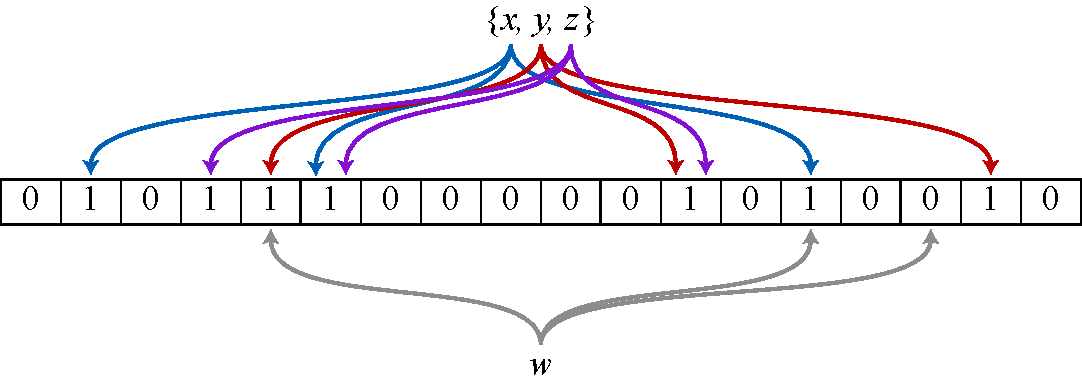
\includegraphics[width=0.8\textwidth]{graphics/bloomfilter.pdf}
				\caption{Bloom filter operation with $m=18$ and $k=3$}
				\label{fig:bloom-filter}
		\end{figure}
			
		To test membership for an item, feed the item to each hash function. If all the corresponding indexes are $1$, then the item \emph{may} be contained within the filter - if any of them are $0$, then the item is definitely not.
		
		For a given number of entries $s$ and a bit vector of size $m$, we need to use $k$ hash functions such that:
		
		\[
		k = \frac{m}{s} \ln 2
		\]
		
		The error rate is defined as:
		
		\[
		\epsilon = 0.5^k
		\]
		
		In essence, the longer the bit vector, the more accurate the filter becomes - at the expense of increasing space requirements. If $m=\infty$, then there are no false positives - the filter becomes accurate and deterministic (for a fixed set of $k$).
		
		\citet{Swamidass2007} show is that the number of elements within a Bloom Filter can be estimated by:
		
		\[
		E = -n \ln \frac{1-n/n}{k}
		\]

\section{Dependency Analysis Algorithms} \label{sec:runtime/analysis}
	Computing dependency between two operations is of critical importance to this project; an efficient algorithm is important.
	
	The problem statement for dependency analysis is as follows:
	
	Let $i^l_n$ be the set of memory accesses for iteration $n$ in loop $l$. For a memory access $\alpha \in i^l_n$, determine whether there exists a previous iteration such that $\alpha \in i^l_{n-c}$ for some integer $c$. Additionally, for an access $\alpha_i$ and previous access $\alpha_{i-c}$, $kind(\alpha_i) \neq read \wedge kind(\alpha_{i-c}) \neq read$.

	\subsection{Offline Algorithms} \label{sec:runtime/analysis/offline}
	An offline algorithm means that any processing is performed after the trace has been collected \citep[p.~525-526]{TAOCPvol2}. It is the simplest form of dependency analysis algorithm, but it show poor performance. For a number of loops $l$ with an average of $i$ iterations each, where each iteration has an average of $o$ operations, then $T_{offline}=O(lio)$.
	
	\begin{algorithm}
		\caption{Offline dependency algorithm}
		\label{alg:offline-dependency}
		\begin{algorithmic}[1]
			\STATE $d \gets \varnothing$ %\COMMENT{$d$ is the set of dependencies}
			\FORALL{loops $l$}
				\STATE $p \gets \varnothing$ %\COMMENT{$p$ is the set of previous iterations}
				\FORALL{iteration $i \in l$}
					\FORALL{access $\alpha \in i$}
						\FORALL{$p_{\alpha} \in p$}
							\IF{$\alpha \in p{_\alpha}$}
								\STATE $d \gets \alpha$
							\ENDIF
							
							\STATE $p \gets \alpha$
						\ENDFOR
					\ENDFOR
				\ENDFOR
			\ENDFOR
		\end{algorithmic}
	\end{algorithm}
	
	This offline algorithm has several disadvantages. Not only is its runtime particularly poor (we can achieve at least a factor $l$ speed-up using an online algorithm), but because it requires a complete trace of accesses per iteration, it is unsuitable for  detecting dependencies at run-time. Algorithm \ref{alg:offline-dependency} outlines the offline algorithm.

	\subsection{Online Algorithns} \label{sec:runtime/analysis/online}
	\begin{figure}
			\centering
			\begin{tikzpicture}[->,>=stealth',shorten >=1pt,auto,node distance=3.5cm,semithick, bend angle=35]
				\node[initial,accepting,state]	(q1)					{$S$};
				\node[state]					(q2)	[right of=q1]	{$Q$};
				
				\path[->]
					(q1)	edge [bend left ] node {loop begin} (q2)
					(q2)	edge [bend left] node {loop stop} (q1)
							edge [loop right] node {iteration} (q2);
					
			\end{tikzpicture}
			\caption{Finite state machine for the online algorithm}
			\label{fig:online-fsm}
		\end{figure}
		
	An online algorithm for this problem is one that runs with a sequential input of values. An online algorithm is superior because it shows better performance characteristics asymptotically, $T_{online} = O(io)$, and it runs in conjunction with the program. This allows Locomotion, in theory, to advice any JIT compilers of optimisations to perform. Figure \ref{fig:online-fsm} represents the finite state machine for the algorithm.
	
	\begin{algorithm}
		\caption{Online dependency algorithm}
		\label{alg:online-dependency}
		\begin{algorithmic}
			\STATE something
		\end{algorithmic}
	\end{algorithm}

\section{Implementation Details} \label{sec:runtime/implementation}
\